\section{Istruzioni per l'utilizzo}
\subsection{Autenticazione}
All'avvio verrà mostrata una schermata che servirà ad autenticarsi, nella quale bisognerà inserire nome utente e password del proprio account \gloman{Zextras Drive}. In caso di successo dell'operazione si avvierà il \gloman{software}, altrimenti verrà visualizzato un messaggio di errore e chiesto di reinserire le credenziali.
\begin{figure}[H]
    \centering
    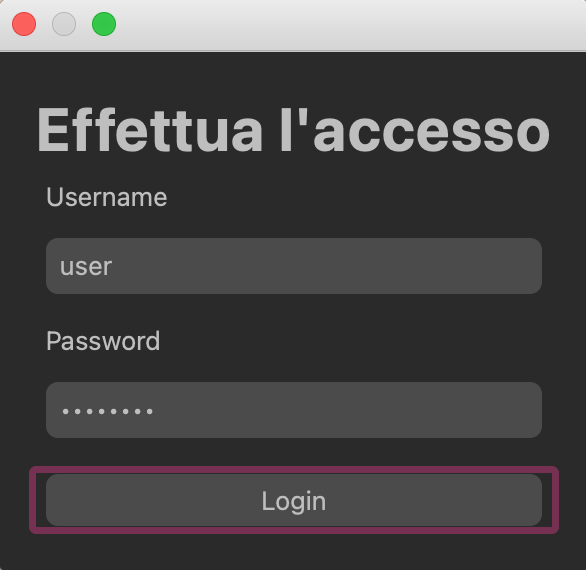
\includegraphics[scale = 0.50]{components/img/login.png}
    \caption{Vista del login}
    \label{fig:Vista del login}
\end{figure}
\subsection{Selezione del percorso da sincronizzare}
\label{sec:selezionepath}
Al primo avvio dell'applicazione verrà richiesto di scegliere una cartella, nella quale verranno sincronizzati tutti i file. Non si deve scegliere la stessa cartella nella quale è contenuto il programma.
\begin{figure}[H]
    \centering
    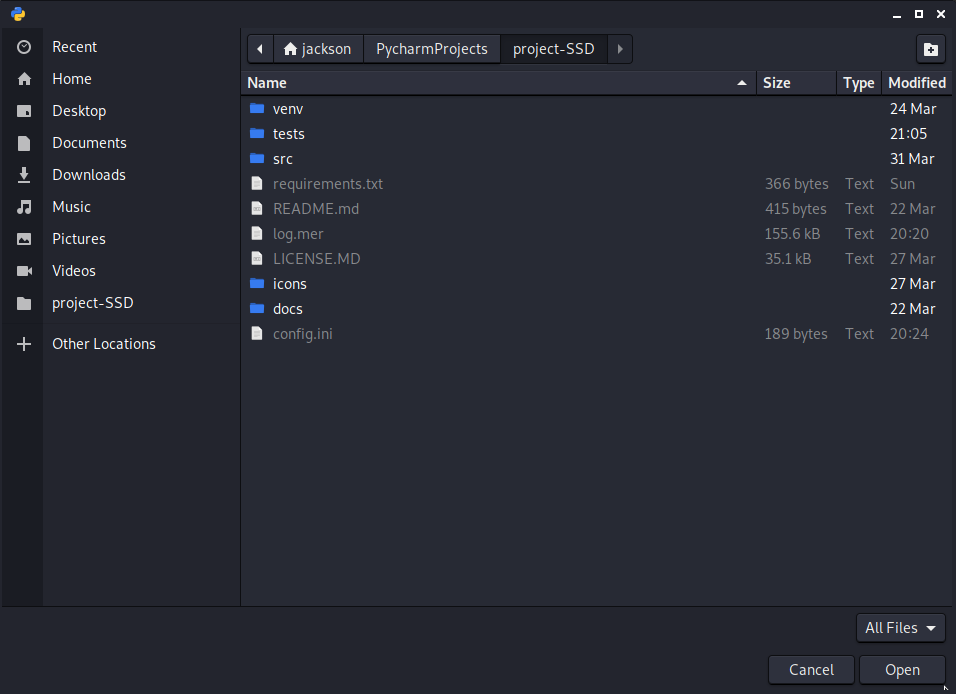
\includegraphics[scale = 0.30]{components/img/selezione-path.png}
    \caption{Selezione del percorso da sincronizzare}
    \label{fig:Selezione del percorso da sincronizzare}
\end{figure}

\subsection{Visualizzazione file nel percorso scelto}
\begin{figure}[H]
    \centering
    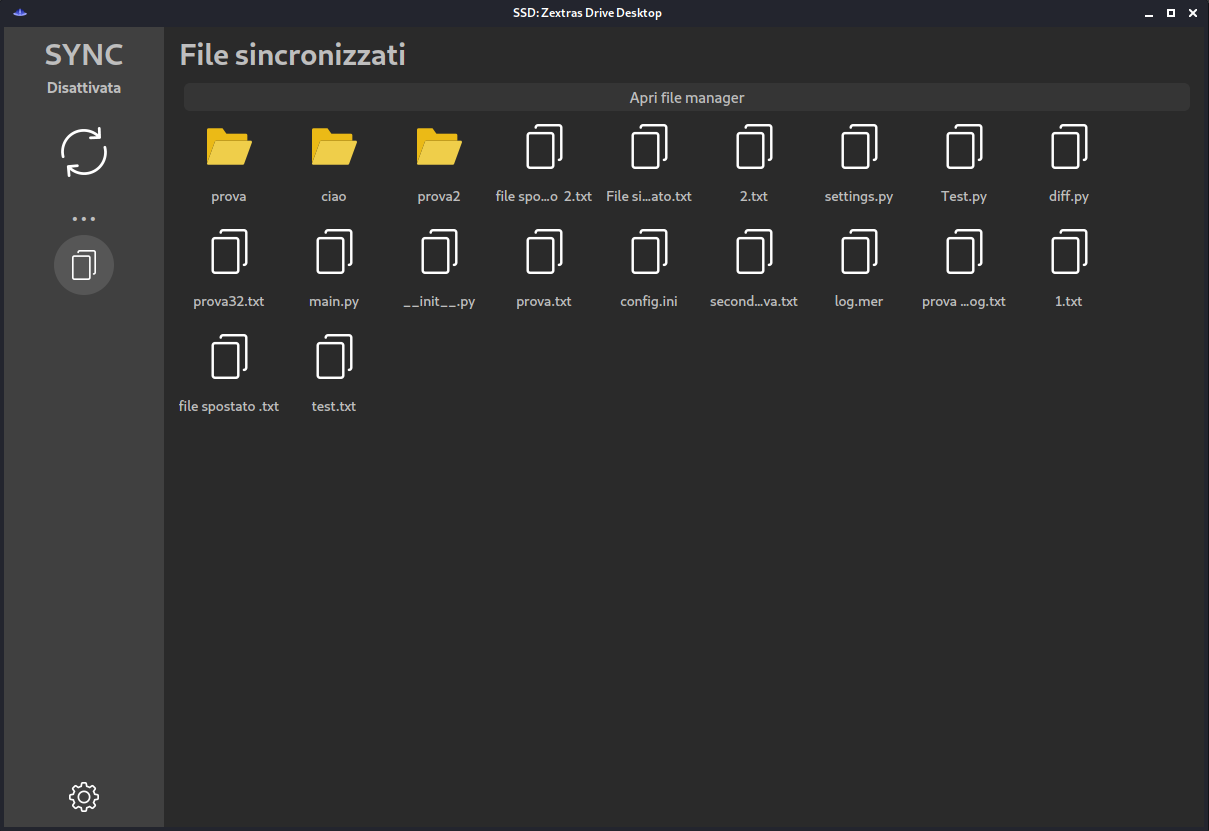
\includegraphics[scale = 0.30]{components/img/file-view.png}
    \caption{Vista dei file nella cartella scelta}
    \label{fig:Vista dei file nel percorso scelto}
\end{figure}
\begin{enumerate}
	\item Pulsante utilizzato per aprire l'esplora risorse del proprio sistema operativo nella cartella attuale;
	\item Pulsante per attivare o disattivare la sincronizzazione della cartella selezionata;
	\item Pulsante per visualizzare i file nel percorso scelto;
	\item Pulsante per aprire la vista di impostazioni (maggiori informazioni a \S{}\ref{sec:impostazioni}).
\end{enumerate}

\subsection{Impostazioni} \label{sec:impostazioni}
\begin{figure}[H]
    \centering
    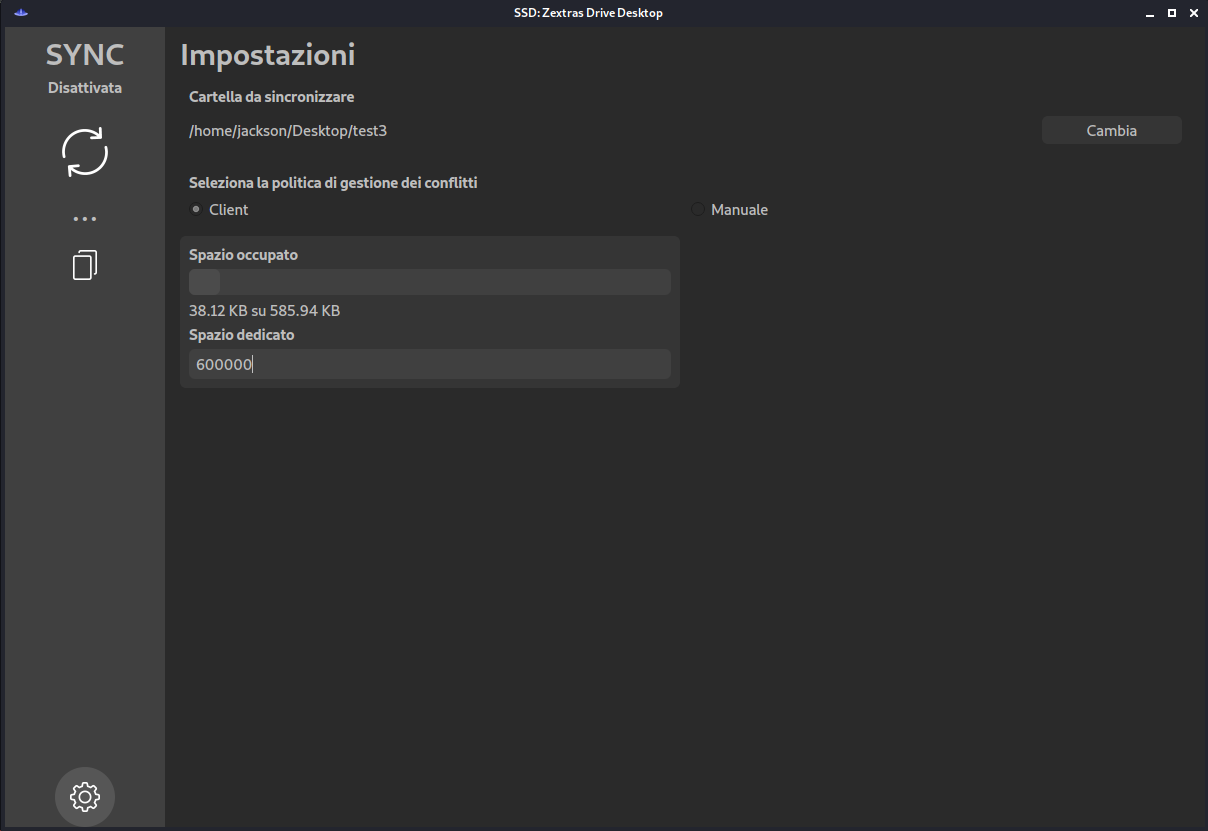
\includegraphics[scale = 0.30]{components/img/settings.png}
    \caption{Vista delle impostazioni}
    \label{fig:Vista delle impostazioni}
\end{figure}
\begin{enumerate}
	\item Pulsante utilizzato per cambiare il percorso della cartella sincronizzata (maggiori informazioni a \S{}\ref{sec:selezionepath});
	\item Pulsanti mutualmente esclusivi, il pulsante premuto indica la politica di sincronizzazione:
	\begin{itemize}
		\item \textbf{Client}: questa politica di sincronizzazione dà la priorità ai file locali. Se un file è stato modificato nel \gloman{server} e nel \gloman{client}, la priorità viene data al file presente in locale, che verrà caricato nel \gloman{server};
		\item \textbf{Manuale}: questa politica di sincronizzazione richiede l'interazione dell'utente in caso di \gloman{conflitto} tra file nel \gloman{server} e file nella cartella locale.
	\end{itemize}
	\item Barra indicante lo spazio occupato. Viene mostrato graficamente quanto spazio la cartella da sincronizzare selezionata pesa sullo spazio riservato nel punto 4;
	\item Campo utilizzato per impostare quanto spazio del disco locale può essere occupato al massimo dal programma di sincronizzazione.
\end{enumerate}